%
% $RCSfile: conglomerate.tex,v $
%
% Copyright (C) 2002-2008. Christian Heller.
%
% Permission is granted to copy, distribute and/or modify this document
% under the terms of the GNU Free Documentation License, Version 1.1 or
% any later version published by the Free Software Foundation; with no
% Invariant Sections, with no Front-Cover Texts and with no Back-Cover
% Texts. A copy of the license is included in the section entitled
% "GNU Free Documentation License".
%
% http://www.cybop.net
% - Cybernetics Oriented Programming -
%
% http://www.resmedicinae.org
% - Information in Medicine -
%
% Version: $Revision: 1.1 $ $Date: 2008-08-19 20:41:06 $ $Author: christian $
% Authors: Christian Heller <christian.heller@tuxtax.de>
%

\subsection{Conglomerate}
\label{conglomerate_heading}
\index{Universe as Conglomerate}

\emph{Universe} is the most general word describing everything humans think
exists. Whether it exists in reality or just as an illusion in their minds, is
a fundamental question of philosophy and will not be discussed here. The author
of this document assumes that a \emph{Real World} exists and humans only
\emph{reflect} but not \emph{construct} it in their minds.

\begin{figure}[ht]
    \begin{center}
        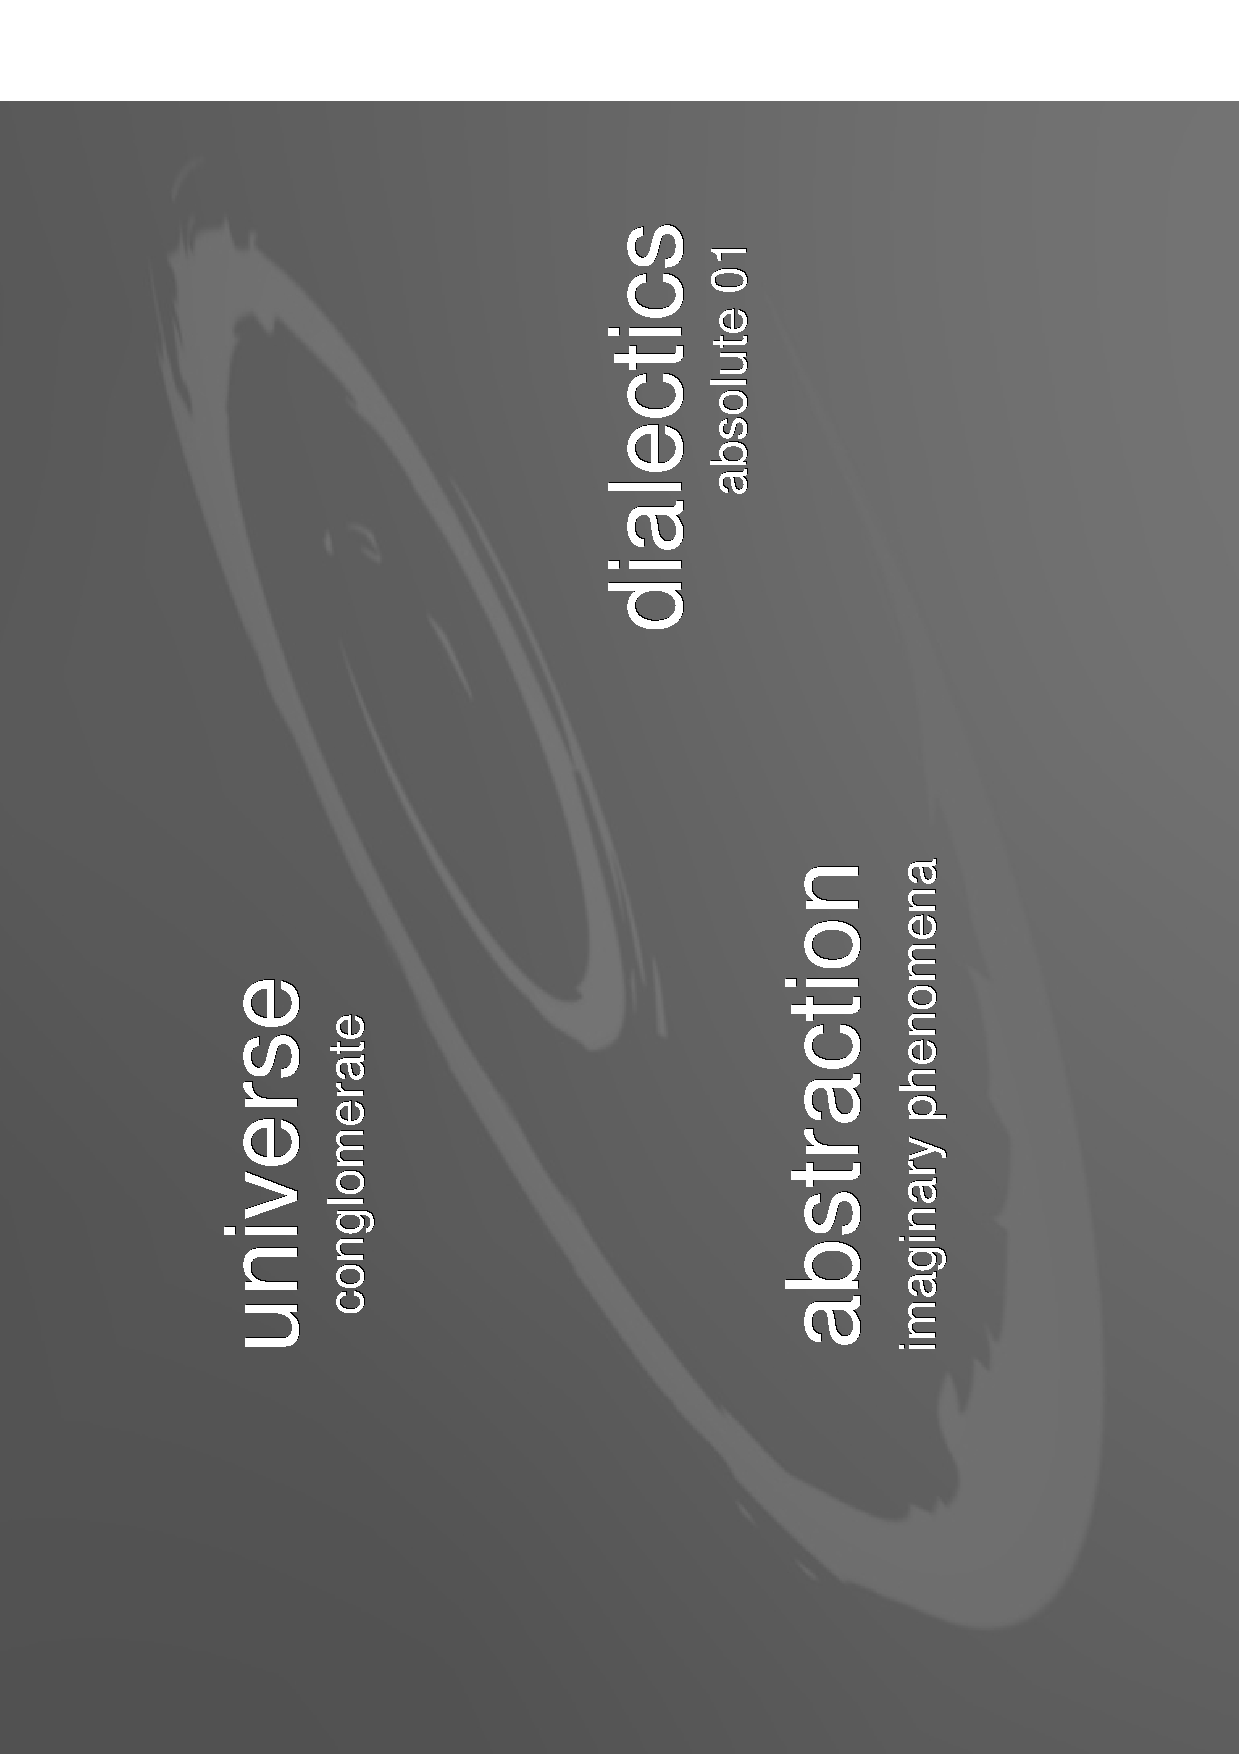
\includegraphics[scale=0.3,angle=-90]{graphic/conglomerate.pdf}
        \caption{The Universe as to-be-abstracted Conglomerate (swirl from \cite{debian})}
        \label{conglomerate_figure}
    \end{center}
\end{figure}

The whole universe can be seen as \emph{Conglomerate} of everything in
existence (figure \ref{conglomerate_figure}). Computer systems enable humans to
abstract things to just two states labelled \emph{0} and \emph{1} (section
\ref{hardware_architecture_heading}), on a very low level. Human systems use
more high-level methods for abstraction. Common concepts to describe a
real-world environment are \emph{Particle}, \emph{Dimension} or \emph{Force}.
Everybody will know more of them. But what is a particle?
